\documentclass[border=4pt]{standalone}
\usepackage{fontspec}
\usepackage{amsmath}
\usepackage{unicode-math}
\setmainfont{Latin Modern Roman}
\setmathfont{Latin Modern Math}
\usepackage{pgfplots}
\usepackage{pgfplotstable}
\pgfplotsset{compat=1.18}
\usepackage{tkz-euclide}
\usetikzlibrary{arrows.meta,calc,angles,quotes,patterns,3d,backgrounds}
\definecolor{ink}{HTML}{123428}
\definecolor{asy}{HTML}{475569}
\definecolor{mint}{HTML}{86e0bd}
\tikzset{asym/.style={asy, line width=0.9pt, dash pattern=on 5pt off 3.5pt},
         guide/.style={gray!70, line width=0.6pt, densely dotted},
         dot/.style={circle, inner sep=0pt, minimum size=5pt, draw=white, line width=0.5pt},
         odot/.style={circle, inner sep=0pt, minimum size=5.5pt, fill=white, line width=1pt},
         lab/.style={font=\footnotesize, inner sep=1.5pt, text=ink}}
\begin{document}
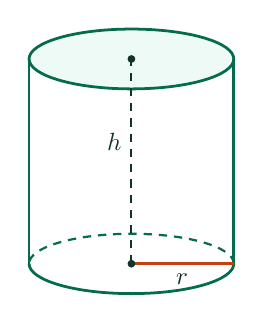
\begin{tikzpicture}[line join=round]
\draw[color={rgb,255:red,4;green,107;blue,77}, line width=1pt] (-1.3,0) arc[start angle=180, end angle=360, x radius=1.3cm, y radius=0.38cm];
\draw[color={rgb,255:red,4;green,107;blue,77}, line width=0.8pt, dash pattern=on 3pt off 2.5pt] (1.3,0) arc[start angle=0, end angle=180, x radius=1.3cm, y radius=0.38cm];
\draw[color={rgb,255:red,4;green,107;blue,77}, line width=1pt, fill={rgb,255:red,134;green,224;blue,189}, fill opacity=0.15] (0,2.6) ellipse (1.3cm and 0.38cm);
\draw[color={rgb,255:red,4;green,107;blue,77}, line width=1pt] (-1.3,0) -- (-1.3,2.6) (1.3,0) -- (1.3,2.6);
\draw[ink, line width=0.7pt, dash pattern=on 3pt off 2.5pt] (0,0) -- (0,2.6);
\draw[color={rgb,255:red,194;green,65;blue,12}, line width=1pt] (0,0) -- (1.3,0);
\fill[ink] (0,0) circle (1.4pt); \fill[ink] (0,2.6) circle (1.4pt);
\node[font=\small, text=ink, below] at (0.65,0) {$r$};
\node[font=\small, text=ink, left] at (0,1.55) {$h$};
\end{tikzpicture}
\end{document}
